\documentclass[12pt,a4paper]{article}
\usepackage[utf8]{inputenc}
\usepackage[english,russian]{babel}
\usepackage{indentfirst}
\usepackage{misccorr}
\usepackage{graphicx}
\usepackage{amssymb}
\usepackage{amsmath}

\begin{document}

\begin{center}
    \large
    Работа 1.4.2
    
    Сибгатуллин Булат, Б01-007
    
    \vspace{0.5cm}
    \textbf{Определение ускорения свободного падения при помощи оборотного маятника}

\end{center}

\vspace{0.5cm}
\textbf{Цель работы:} определить величину ускорения маятника свободного падения, пользуясь оборотным маятником.
    
\vspace{0.5cm}
\textbf{В работе используются:} оборотный маятник, счетчик числа колебанийб секундомерб штангенцирекль с пределом измерений 1 $\textit{м}$.

\vspace{0.5cm}

Свободным падением называют движение тела вблизи поверхности Земли, при котором модно не учитывать силы сопротивления, возникающие в среде окружающей тело. Ускорение свободного падени вблизи поверхности Земли можем рассчитать по формуле:

\begin{equation}\label{1}
    \Vec{g} = \frac{\Vec{F}}{m}
\end{equation}

Система отсчета, связанная с Землей, не является инерциальной. В этой системе на тело, кроме гравитационных сил, действуют ещё центробежная сила и сила Кориолиса. Под ускорением свободного падения обычно понимается тангенциальная к траектории компонента ускорения, и сила Кориолиоса при этом не учитывается. Очевидно, что для покоящегося на поверхности Земли тела сумма силы притяжения к Земле и центробежной равна силе реакции опоры, то есть весу тела.

Сила притяжения тела к Земле определяется произведением его массы 
\begin{math}
    m
\end{math}
на напряженность поля тяготения Земли, которая обычно обозначается 
\begin{math}
    \Vec{g_0}
\end{math}
:

\begin{equation}\label{2}
    \Vec{F_0} = m\Vec{g_0}
\end{equation}

Напряженность поля тяготения определяется распределением масс в Земле. Если бы Змеля представляла собой шар постоянной плотности, то внутри шара напряженность росла пропорционально расстоянию от центра Земли, а вне шара падала бы обратно пропорционально квадрату расстояния от центра Земли. В действительности Земля не очень однородна. Плотность её растёт с глубиной. Из-за этого напряженность поля тяготения даже немного увеличивается с глубиной, примерно до 2800 $\textit{км}$ (при этом расстояние до центра Земли около 3600 $\textit{км}$), а затем начинает падать по линейному закону. Над поверхностью Земли распределение напряженности гравитационного поля близко к распределению вне однородного шара. На пысоте порядка 300 $\textit{км}$ напряженность поля тяготения меньше, чем у поверхности Земли, примерно на 
$10 \textit{\%}\textit{.}$

Кроме сил притяжения к Земле, действуют ещё силы притяжения к Луне и Солнцу, но вклад их в полную напряженность гравитационного поля очень мал, хотя они в глобальных масштабах вызыва.т такие заметные явления, как приливы.

Вращение Земли привело к её деформации за счёт центробежных сил. Суммарная напряженность поля,обозначаемая 
\begin{math}
    g
\end{math}
и равная ускорению свободного падения, обычно приводится в таблицах распределения свободного падения по поверхности Земли. На полюсе $g = 983,2155$ $  \textit{см}/\textit{с}^2$, а затем умеьшается с уменьшением широты, и на экваторе $g = 978,0300$ $  \textit{см}/\textit{с}^2$. Это приводит, например к тому, что маятниковые часы на экваторе за сутки отстанут от аналогичных часов на полюсе на 3,8 минуты.

Неоднородность Земли в горизонтальном направлении также приводит к локальным изменениям $g$. Большое количество очень точных измерений на поверхности Земли показало, что $g$ менятся также со временем. Периодические изменения, связанные с лунными приливами, равны примерно $2,49\cdot10^{-4}$ $\textit{см}/\textit{с}^2$, а с солнечными - порядка $9,6\cdot10^{-5}$ $\textit{см}/\textit{с}^2$. Такого же порядка изменения происходящиев течение года, связаны с геологическими процессами внутри Земли (так называемые вековые изменения.

Первые измерения $g$ с точностью до $10^{-3}$ $\textit{см}/\textit{с}^2$ (миллигал) были выполнены в начале века с помощью оборотных маятников. Для получения такой точности периоды колебаний должны быть измерены с точностью до $10^{-6}$ $\textit{с}$, а приведенные длины - до 1 микрона. Современные методы измерения полей $g$ делятся на динамические и статические. К динамическим относятся измерения с помощью маятников, в том числе и оборотных.

В последнее время благодаря увеличению точности измерений расстояний и времен стали применяться прямые методы измерения ускорения падающих тел. Использование лазерных интерферометров для измерения пути падающего в вакуумной трубе тела, снабженного уголковым отражателем, и атомных часов позволило определить абсолютное значение ускорения свободного падения с точностью до $3\cdot10^{-6}$ $\textit{см}/\textit{с}^2$. Динамические методы позволяют измерять абсолютные значения ускорения свободного падения. Статические методы позволяют измерять относительное изменение ускорения свободного подения с точностью до $1,5\cdot10^{-5}$ $\textit{см}/\textit{с}^2$ и основываются на измерении деформации пружин, на которых подвешены грузики, либо на закручивании горизонтально закрепленных нитей под действием рычагов с грузиками.

Период колебаний физического маятника определяется формулой:
\begin{equation}\label{3}
    T = 2\pi\sqrt{\frac{I}{mga}}
\end{equation}

Здесь $I$ - момент инерции маятника относительно оси качания, $m$ - масса маятника, $a$ - расстояние от центра масс до оси качания.

Приведенная длина физического маятника, равная длине математического маятника, имеющего такой же период колебаний, выражается формулой:
\begin{equation}\label{4}
    l_{pr} = \frac{I}{ma}
\end{equation}

Массу маятника и период его колебаний можно измерить с высокой точностью, но точно измерить момент инерции не удается. Указанного недостатка лишен метод оборотного маятника, который позволяется исключить момент инерции из расчетной формулы для $g$.

Метод оборотного маятника основан на том, что период колебаний физического маятника не изменяется при перемещении оси в центр качаний, т.е. в точку, отстоящую от оси качаний на расстояние, равное приведенной длине маятника, и лежащую на одной прямой с точкой подвеса и центром масс маятника.

\begin{figure}[h!]
\centering
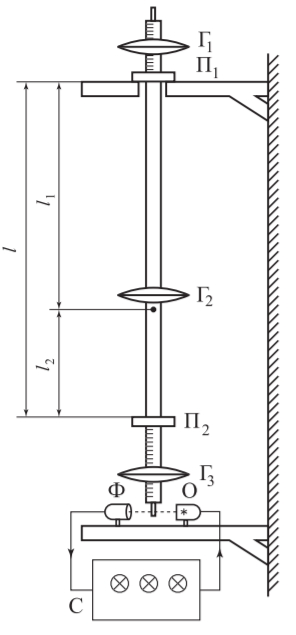
\includegraphics[scale=1]{Image1.png}
\caption{Оборотный маятник}
\label{fig:Image1}
\end{figure}

Применяемый в настоящей работе оборотный маятник (рис. 1) состоит из стальной пластины (или стержня), на которой укреплены две однородные призмы П$_1$ и П$_2$. Период колебаний маятника можно менять при помощи подвижных грузов Г$_1$, Г$_2$ и Г$_3$.

Допустим, что нам удалось найти такое положение грузов, при котором периоды колебаний маятника $T_1$ и $T_2$ на призмах П$_1$ и П$_2$ совпадают, т.е.
\begin{equation}\label{5}
    T_1 = T_2 = 2\pi\sqrt{\frac{I_1}{mgl_1}} = 2\pi\sqrt{\frac{I_2}{mgl_2}},
\end{equation}

где $L_1$ и $L_2$ - расстояния от центра массы маятника до призм П$_1$ и П$_2$.

Условием этого, очевидно, является равенство приведенных длин, т.е. равенство величин $I_1/ml_1^2$ и $I_2/ml_2^2$. По теореме Гюйгенса-Штейнера

\begin{equation}\label{6}
    I_1 = I_0 + ml_1^2, \quad I_1 = I_0 + ml_1^2,
\end{equation}

где $I_0$ - момент инерции маятника относительно оси, проходящей через его центр масс (и параллельной оси качаний). Исключая из (\ref{5}) и (\ref{6}) $I_0$ и  $m$, получим формулу для определения $g$:

\begin{equation}\label{7}
    g = \frac{4\pi^2}{T^2}(l_1 + l_2) = 4\pi^2\frac{L}{T^2}.
\end{equation}

Здесь $L = l_1 + l_2$ - расстояние между призмами П$_1$ и П$_2$, которое легко может быть измерено с выскокой точностью ($0,1 $ $\textit{мм}$) при помощи большого штангенциркуля (но не путем суммирования измерений $l_1$ и $l_2$, погрешность получения которых в работе велика и составляет несколько миллиметров).

Заметим, что формула(\ref{7}) следует из формул (\ref{5}) и (\ref{6}) лишь при условии, что
\begin{equation}\label{8}
    l_1 \neq l_2;
\end{equation}

так как при $l_1 = l_2$ равенства (\ref{5}) и (\ref{6}) удовлетворяются тождественно.

При выводе формулы (\ref{7}) мы полагали, что $T_1 = T_2$. На самом деле точного равенства добиться, конечно, невозможно. Тогда

\begin{center}
    $T_1 = 2\pi\sqrt{\frac{I_0 + ml_1^2}{mgl_1}}, \quad T_2 = 2\pi\sqrt{\frac{I_0 + ml_2^2}{mgl_2}}.$
\end{center}

Из этих равенств имеем

\begin{center}
    $T_1^2gl_1 - T_2^2gl_2 = 4\pi^2(l_1^2 - l_2^2),$
\end{center}

откуда

\begin{equation}\label{9}
    g = 4\pi^2\frac{l_1^2 - l_2^2}{l_1T_1^2 - l_2T_2^2} = 4\pi\frac{L}{T_0^2},
\end{equation}

где

\begin{equation}\label{10}
    T_0^2 = \frac{l_1T_1^2 - l_2T_2^2}{l_1 - l_2} = T_2^2 + \frac{l_1}{l_1 - l_2}(T_1 + T_2)(T_1 - T_2).
\end{equation}

Погрешность определения $g$ может быть найдена из (\ref{9}):

\begin{equation}\label{11}
    \frac{\sigma_g}{g} = \sqrt{\Big(\frac{\sigma_L}{L}\Big)^2 + 4\Big(\frac{\sigma_{T_0}}{T_0}\Big)^2}.
\end{equation}

Входящая в эту формулу погрешность $\sigma_{T_0}$ сама должна быть вычислена. Прежде чем это сделать, исследуем, как зависит период колебаний от расстояния $l$ между центром масс и осью качаний маятника. Для этого выразим момент инерции $I$ с помощью (\ref{6}) через $I_0$:

\begin{equation}\label{12}
    T = 2\pi\sqrt{\frac{I_0 + ml^2}{mgl}}.
\end{equation}

График этой зависимости изображен на рис. 2. При $l \to 0$ период $T$ стремится к бесконечности по закону $l^{-1/2}$. При $l\to\infty$ он стремится к бесконечности как $l^{1/2}$. Период минимален при двух разных значениях $l$: одно из них больше, а другое меньше $l_{min}$. Эти разные значения и были использованы в формулах (\ref{5}) - (\ref{7}). Из графика видно , что при изменении $T$ величины $l_1, l_2$ сближаются или удаляются друг от друга.

\begin{figure}[h!]
\centering
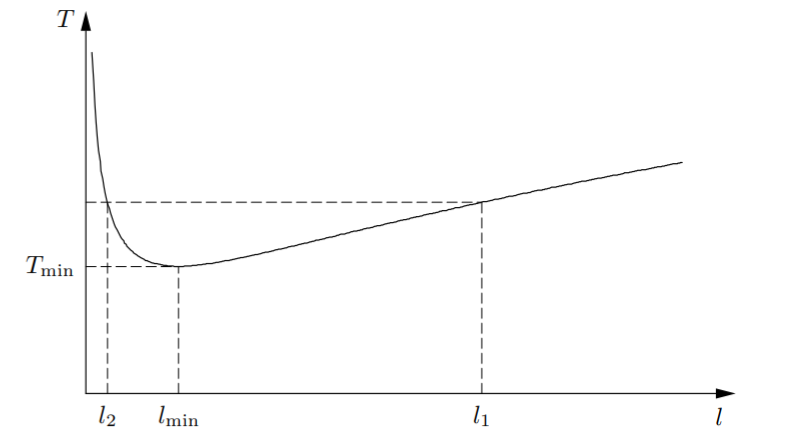
\includegraphics[scale=1]{Image2.png}
\caption{Зависимость периода колебания маятника от расстояния между центром масс и осью качаний}
\label{fig:Image2}
\end{figure}

Найдем зависимость погрешности в определении $T_0$ от разности $l_1-l_2$. Для этого исследуем, например, как завсити $\sigma_{T_0}$ от погрешности в поределении $T_1$. Дифференцируя первое равенство (\ref{10}) и полагая $T_2$ неизменным, мы получаем

\begin{center}
    $2T_0(dT_0)_{T_2} = \frac{l_1}{l_1-l_2}2T_1dT_1, \quad (dT_0)_{T_2} = \frac{l_1}{l_1-l_2}\cdot\frac{T_2}{T_0}dT_1.$
\end{center}

Аналогично при неизменном $T_1$ получим

\begin{center}
    $(dT_0)_{T_1} = -\frac{l_2}{l_1-l_2}\cdot\frac{T_2}{T_0}dT_2.$
\end{center}

Рассмотрим случай, когда $l_1$ и $l_2$ близки друг к другу.Знаменатель формулы при этом мал и погрешность в определении $T_0$ резко возрастает. Тот же вывод справедлив для пересчета погрешности $dT_2$ в погрешность $dT_0$ (при неизменном $T_1$). Поэтому период колебаний следует выбирать так, чтобы $l_1$ и $l_2$ заметно отличались друг от друга (при различии их в 1,5 раза погрешность $T_0$ превышает погрешность $T_1$ менее чем на порядок).

Получим формулу для расчета погрешности $dT_0$. Обратимся для этого ко второму равенству (\ref{10}). Заметим, что $T_1\approx T_2$, так что $T_1 - T_2$ мало. Поэтому при не слишком малых $l_1-l_2$ второй член в этой формуле играет роль небольшой поправки.

Следовательно, если учитывать ошибки измерений $l_1$ и $l_2$ (но не $T_1$ и $T_2$), то эти ошибки будут умножаться на малую величину $T_1 - T_2$ и ими при расчете погрешностей $\sigma_{T_0}$ можно пренебречь (даже несмотря на то, что эти ошибки могут быть равны нескольким миллиметрам, что обычно получается в данной работе). Учитывая, что погрешностии в измерении периодов $T_1$ и $T_2$ независимы и примерно равны друг другу, окончательно найдем, используя для расчета ошибок общую формулу:

\begin{equation}\label{13}
    \sigma_{T_0}\approx\frac{\sqrt{l_1^2+l_2^2}}{l_1-l_2}\sigma_T,
\end{equation}

где $\sigma_T$ - погрешность измерений периодов.

Видно, что погрешность периодов слабо зависит от точности с которой выпонятеся $T_1 = T_2$. Поэтому нет смысла тратить время на его уточнение, когда они равны друг другу, с точностью до нескольких процентов.

Заметим, наконец, что соотношение $l_1/l_2$ не должно быть слишком большим. При увеличении их отношения, увеличивается время измерения и растет роль сил трения, которые при выводе формулы (\ref{3}) не учитывались.

Поясним это утверждение. Роль трения определяется отношением работы, производимой этими силами за период колебаний, к запасу колебательной энергии в системе. Работа сио трения слабо зависит от $l_2$. Запас колебательной энергии равен потенциальной энергии, которую приобретает маятник при поднятии его центра масс, т.е.

\begin{center}
    $W_{hes} = mgl_2(1-\cos\varphi),$
\end{center}

где $\varphi$ - угол отклонения маятника. При уменьшение $l_2$ значение $W_hes$ падает. Таким образом, мы приходим к выводу, что отношение $l_1$ к $l_2$ не должно быть ни слишком большим; желательно, чтобы выполнялось условие
\begin{equation}\label{14}
    1,5<\frac{l_1}{l_2}<3.
\end{equation}

\vspace{1cm}

\large\textbf{Ход работы}

\vspace{1cm}

\textbf{1.} Познакомимся с прибором и оборотным маятником. Определим из характеристик прибора его погрешность $\sigma_t = 0,01 (\textit{с})$.
Определим рабочий диапазон амплитуд, в пределах которого период колебаний \textit{T} можно считать не зависящим от амплитуды. Для этого установив маятник на одной из призм и отклонив его на угол $\varphi (\sim 10^{\circ})$, и измерим время 100 полных колебаний. Уменьшим угол отклонения в два раза и повторим измерения в результате получив период $\textit{T'}$.

Получим \textit{T} = $151,67  / 100 = 1,5167$ \textit{с}, $\textit{T'} = 151,45 / 100 = 1,5145$ \textit{с}. В пределах точности измерений получаем $\textit{T} = \textit{T'}$.

\vspace{0,5cm}

\textbf{2.} Изучим каким образом время колебаний $\textit{T}_1$ и $\textit{T}_2$ (при опоре на призмы $\textit{П}_1$ и $\textit{П}_2$ соответсвенно) зависят от положения грузов $\textit{Г}_1$, $\textit{Г}_2$ и $\textit{Г}_3$. Изначально грузы $\textit{Г}_1$ и $\textit{Г}_3$ вплотную прижаты к соответствующим призмам.

\vspace{0,5cm}

\begin{center}
\begin{tabular}{|c|c|c|c|c|c|}
\hline 
$\textit{T}_1$ & 1,531 & 1,527 & 1,537 & 1,534 & 1,526 \\ 
\hline 
$\textit{T}_2$ & 1,517 & 1,507 & 1,527 & 1,523 & 1,509 \\ 
\hline 
\end{tabular} 
\end{center}

\vspace{0,5cm}

В данной таблице первый столбик (не считаю столбца с обозначениями $\textit{T}_1$ И $\textit{T}_1$) включает в себя информацию о периодах в начальный момент времени. Второй столбец задает информацию о периодах при $\textit{Г}_2$ смещенном в сторону $\textit{Г}_1$, третий при $\textit{Г}_2$ смещенном в сторону $\textit{Г}_3$, четвертый при $\textit{Г}_1$ смещенном в сторону от $\textit{Г}_1$ и пятый при $\textit{Г}_3$ смещенном в сторону от $\textit{Г}_1$.

По результатам измерений можем определить, что на изменение $\textit{T}_1$ в большей степени влияет перемещение $\textit{Г}_1$. На изменение $\textit{T}_2$ в большей степени влияет перемещение $\textit{Г}_3$. А на изменение $\vert\textit{T}_1 - \textit{T}_2\vert$ в большей степени влияет перемещение $\textit{Г}_2$. При чем при перемещении $\textit{Г}_1$ и $\textit{Г}_3$ периоды $\textit{T}_1$ и $\textit{T}_2$ изменяются в одну сторону, а при перемещении $\textit{Г}_2$ в разные.

\vspace{0,5cm}

\textbf{3.} Перемещая груз наиболее сильно влияющий на величину разности (в нашем случае это $\textit{Г}_2$) добьемся грубого совпадения периодов. В результате получим $\textit{T}_1 = 1,532$ и $\textit{T}_2 = 1,522$, тогда $\vert\textit{T}_1 - \textit{T}_2\vert = 0,010$. Проверим, удовлетворяют ли в этом случае $\textit{l}_1$ и $\textit{l}_2$ неравенству (\ref{14}): 

$\textit{l} = 60,00\pm0,01$ (\textit{мм})

$\textit{l}_1 = 37,4\pm0,1$ (\textit{мм})

$\textit{l}_2 = 22,5\pm0,1$ (\textit{мм})

В таком случае:

\[ \frac{l_1}{l_2} = \frac{37,4}{22,5} = 1,66. \]

Следовательно $\textit{l}_1$ и $\textit{l}_2$ удовлетворяют неравенству (\ref{14}).

Перемещая $\textit{Г}_1$ и $\textit{Г}_3$ добьемся более точного совпадения $\textit{T}_1$ и $\textit{T}_2$. В результате получим $\textit{T}_1 = 1,537$ и $\textit{T}_2 = 1,529$, тогда $\vert\textit{T}_1 - \textit{T}_2\vert = 0,007$. Проверим, удовлетворяют ли для данных значений периода неравенство (\ref{14}):

$\textit{l}_1 = 36,2\pm0,1$ (\textit{мм})

$\textit{l}_2 = 23,8\pm0,1$ (\textit{мм})

В таком случае:

\[\frac{l_1}{l_2} = \frac{36,2}{23,8} = 1,52.\]

Следовательно $\textit{l}_1$ и $\textit{l}_2$ удовлетворяют неравенству (\ref{14}).

Окончательное измерение величин проведу по \textit{N} = 250 полным колебаниям маятника. Также убежусь в том, что трение не оказывает заметного влияния на колебания (за 250 раз амплитуда колебания заметно не иззменяется).

Для 250 колебаний получаем, что $\textit{T}_1 = 1,538$ и $\textit{T}_2 = 1,531$, тогда  $\vert\textit{T}_1 - \textit{T}_2\vert = 0,008$. По результатам измерений можем убедиться, что трение не оказывает существенного влияния на колебания.

\vspace{0,5cm}

\textbf{4.} Проведя все нужные измерения вычислим ускорение свободного падения \textit{g} и её погрешность $\sigma_g$. Для того, чтобы вычислить \textit{g} вычислим $\textit{T}_0$ по формуле (\ref{10}), а потом и само ускорение свободного падения:

\[T_0^2 = 1,529^2 +\frac{36,2}{36,2-23,8}(1,537 +1,529)(1,537 - 1,529) = 2,41\: \textit{с}^2\]

\[g = 4\pi^2\frac{0,6}{2,41} = 9,828\: \textit{м}/\textit{с}^2\]

Определим погрешность измерения периодов:

\[\sigma_T =  \frac{\sigma_t}{N} = \frac{0,01}{250} = 0,00004 \: \textit{с}\]

Зная $\sigma_T$ найдем по формуле (\ref{13}) погрешность $\sigma_{T_0}$:

\[\sigma_{T_0} \approx 0,00004\frac{\sqrt{36,2^2 + 23,8^2}}{36,2-23,8} = 0,00014\: \textit{с}\] 

И по формуле \ref{11} окончательно вычислим $\sigma_g$:

\[\sigma_g = g \sqrt{\frac{\sigma_l}{l} + 4 \frac{\sigma_{T_0}}{T_0}}\] 

\[\sigma_g = g \sqrt{\frac{0,1}{600} + 4 \frac{0,00014}{1,552}} = 0,023\: \textit{м}/\textit{с}^2\]

По полученным данным $g = 9,828\pm0,023\: \textit{м}/\textit{с}^2$.

\vspace{0,5cm}

Сравним полученные данные с табличными значением на данной широте. Стандартное значение ускорение свободного падения составляет 9,815 $\textit{м}/\textit{с}^2$, это значение совпадает с полученными нами данными в пределах погрешности.

Оценим влияние луны на ускорение свободного падения масса луны $m = 7,3477 \cdot 10^{22}$ \textit{кг}, расстояние от Земли до луны равно $l = 3,844 \cdot 10^8$ \textit{м}. Наибольшая разница в измерениях ускорения свободного падения вызванная влиянием луны будет достигаться когда вначале луна будет находиться над нами, а потом под (в надире). Эту разницу можно посчитать по формуле:

\[\delta g = 2\frac{F}{m} = 2\frac{Gm}{l^2}\]

\[\delta g = 6,633 \cdot 10^{-5} \: \textit{м}/\textit{с}^2\]

Эта разница гораздо меньше, чем точность с которой мы измерили ускорение свободного падения.  Следовательно, в нашем случае мы не сможем заметить влияние луны на ускорение свободного падения.

\textbf{Вывод:} познакомились с обротным маятником, с его помощью с высокой точностью определили величину ускорения свободного падения.

\end{document}
